\documentclass[10pt,letterpaper]{article}
\usepackage[margin=1in]{geometry}
\usepackage[latin1]{inputenc}
\usepackage{amsmath}
\usepackage{amsfonts}
\usepackage{amssymb}
\usepackage{graphicx}
\usepackage{hyperref}
\usepackage[nolist,nohyperlinks]{acronym}
\usepackage{float}
\usepackage{subcaption}

\newacro{TR}{Transition Region}
\newacro{EE}{Explosive Event}
\newacro{CT}{Computed Tomography}
\newacro{CTIS}{Computed Tomography Imaging Spectroscopy}
\newacro{MOSES}{\textit{Multi-order Solar EUV Spectrograph}}
\newacro{ESIS}{\textit{EUV Snapshot Imaging Spectrograph}}
\newacro{EUV}{extreme ultraviolet}
\newacro{FOV}{field-of-view}
\newacro{CNN}{convolutional neural network}

\title{\textsc{Progress Report: \\ Neural Networks for Computed Tomography Imaging Spectroscopy of the Solar Atmosphere}}
\author{Roy Smart \\ \url{roy.smart@montana.edu} \\ Montana State University, Department of Physics \\ Bozeman, MT 59717, USA}

\begin{document}
	
	\maketitle
	
	\section{Introduction}
	
		The goal of this investigation is to classify \acp{EE} in the solar \ac{TR} using snapshot imaging spectroscopy. 
		We proposed to accomplish this goal using observations from two snapshot imaging spectrographs, the \ac{MOSES}, and the \ac{ESIS}, of which \ac{MOSES} has successfully flown in 2006 and 2015, and \ac{ESIS} is scheduled to launch alongside \ac{MOSES} in 2019.
		
		These spectrographs are unique in that they have the capability to spectrally-resolve a few \ac{EUV} emission lines over a large 2D \ac{FOV}.
		However, this capability depends on the development of robust inversion algorithms that can interpret the data correctly.
		Therfore, the integral part of our proposal was the development of a \ac{CNN}-based inversion algorithm that used the IRIS Si\,\textsc{iv} 1403 \AA\ spectral observations as a model for the \ac{EUV} emission lines observed by MOSES and ESIS.
		
		During the course of our investigation, we found that achieving a full spectrum inversion superior to those demonstrated in the proposal would require a more sophisticated network than previously anticipated.
		This modification will be discussed in Section \ref{sec_gan}, but we were able to build a useful network using our proposed architecture, a central tendency neural network.
		Instead of reconstructing the full spectrum, this network simply reconstructs the central-tendency (bulk doppler shift), which is a much easier problem to solve.
		Unfortunately, out central-tendency network is easily confounded by spikes in the training set, which necessitated the development of a high-performance image despking routine, discussed in Section \ref{sec_dspk}.
		
	
	\section{Progress Report}
	
		While the development of inversion routines is the most discussed milestone of this investigation, assembling the MOSES and ESIS instruments for flight in 2019 is an important goal of my research group.
		My most significant objective in the instrument assembly is the optical alignment and focus of both ESIS and MOSES. 
		This effort has provided much needed experience using the instruments in this study, which will allow us to be more effective in the development of our inversion routines.
		
		Parallel to the advancement of MOSES and ESIS, I was also involved in the design phase of the FURST mission, which was just accepted in this latest LCAS proposal round.
		The design process of FURST gave me useful experience using optical modeling software, which will allow for the implementation of more sophisticated instrument models in our inversion routine.
	
		\subsection{CTIS Inversion Neural Networks}
		
			As discussed in our proposal, we started by attempting to analyze data from the MOSES I mission in 2006.
			Our goal was to reconstruct the spectrum of the He \textsc{ii} 304 \AA line in the MOSES passband 
			
			
			\subsubsection{Spectrum Inversion Network}
			
				
			
			\subsubsection{Central-tendency Inversion Network}
			
				\begin{figure*}[t!]
					\centering
					\begin{subfigure}[t]{0.5\textwidth}
						\centering
						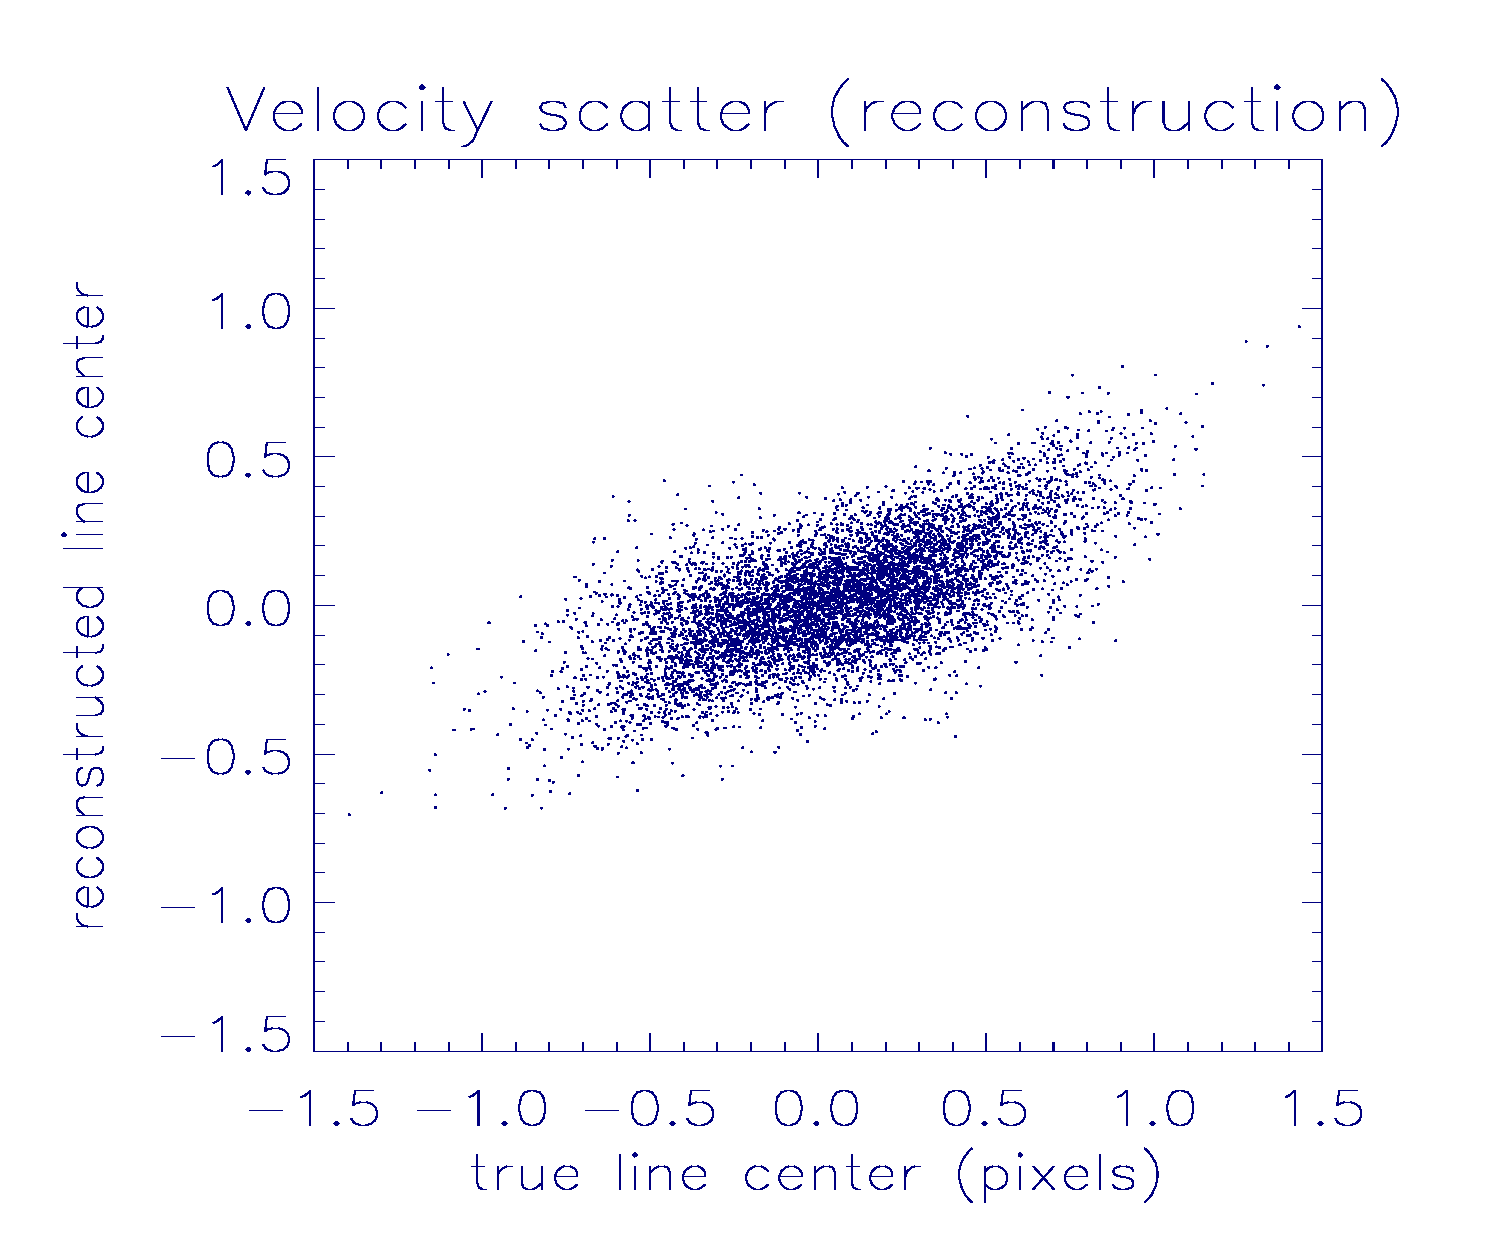
\includegraphics[width=\textwidth]{fig/smart_hist}
						\caption{Lorem ipsum}
					\end{subfigure}%
					~ 
					\begin{subfigure}[t]{0.5\textwidth}
						\centering
						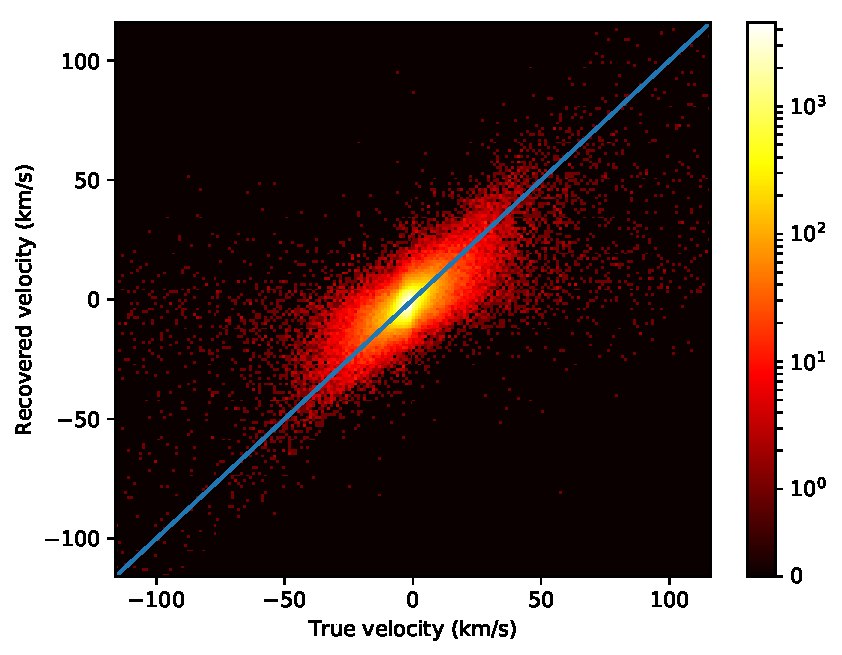
\includegraphics[width=\textwidth]{fig/minnd_hist}
						\caption{Lorem ipsum, lorem ipsum,Lorem ipsum, lorem ipsum,Lorem ipsum}
					\end{subfigure}
					\caption{Caption place holder}
				\end{figure*}
				
				\begin{figure*}[t!]
					\centering
					\begin{subfigure}[t]{0.49\textwidth}
						\centering
						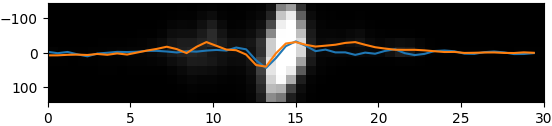
\includegraphics[width=\textwidth]{fig/doppler_1182}
					\end{subfigure}
					~ 
					\begin{subfigure}[t]{0.49\textwidth}
						\centering
						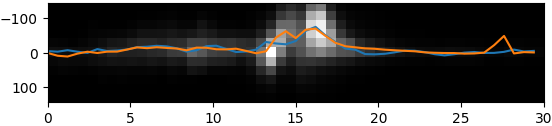
\includegraphics[width=\textwidth]{fig/doppler_1225}
					\end{subfigure}
					~ 
					\begin{subfigure}[t]{0.49\textwidth}
						\centering
						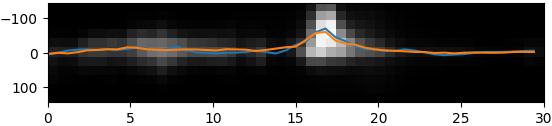
\includegraphics[width=\textwidth]{fig/doppler_1263}
					\end{subfigure}
					~ 
					\begin{subfigure}[t]{0.49\textwidth}
						\centering
						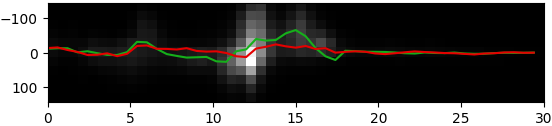
\includegraphics[width=\textwidth]{fig/doppler_1343}
					\end{subfigure}
					\caption{Caption place holder}
				\end{figure*}
				
				
				
			\subsubsection{Despiking Training Data}	\label{sec_dspk}
		
		\subsection{MOSES/ESIS Preparation}
		
		\subsection{FURST Design}
	
	\section{Proposal for Renewal}
	
		\subsection{Further CINN Development}
		
			\subsubsection{Training Data Pipeline}
		
			\subsubsection{Quantile Inversion Network}
			
			\subsection{Generative-Adversarial Networks}	\label{sec_gan}
		
		\subsection{Explosive Event Classification}
		
			
		
		\subsection{MOSES/ESIS Launch}
		
		\subsection{Publications}
	
	\section{Conclusion}
	
\end{document}